\section{Simulación}\label{sec:simulation}

Para comprobar el sistema de control se definió el sistema no-lineal en \Matlab, se obtuvo el sistema lineal sobre un punto de operación tomando el jacobiano del sistema de ecuaciones diferenciales para controlar el sistema, y finalmente se integró el sistema no lineal en el tiempo retroalimentado con el sistema de control.

Se investigó la respuesta del vehículo ante perturbaciones Delta-Dirac de orientación.

\subsection{Sistema no-lineal}

El sistema~\eqref{eq:ssDiffVariables3D} describió la dinámica no-lineal del vehículo con 16 ecuaciones. Estas pudieron ser integradas mediante un método numérico para ecuaciones diferenciales ordinarias multivariables no-autónomas. El requerimiento no-autónomo surgió de la necesidad de incorporar el vector $\Cu$ a la integración, el cual incluyó las actuaciones en base a lo que leyeron los sensores. 

\medskip

Para satisfacer el requerimiento no-autónomo se tuvo que implementar un método numérico basado en Runge-Kutta orden 4. El método fue probado y contrastado con soluciones analíticas conocidas.

\subsection{Sistema de control}

Se optó por controlar mediante el controlador Linear Quadratic Regulator (\gls{lqr}) de la teoría de control óptima debido a la simplicidad de implementación y adaptabilidad para problemas de variables de estado. Como se mencionó anteriormente, se obtuvo el jacobiano del sistema \eqref{eq:ssDiffVariables3D} alrededor del punto de operación. Esta se denominó la matriz del sistema $\MA$. La matriz $\MB$ formó parte del jacobiano del sistema pero diferenciado respecto $\Cu$. Finalmente, $\MC$ resultó la combinación lineal de las mediciones de los sensores (ver sección \ref{sec:model2d} para entender el proceso). 

Se modelaron las siguientes imperfecciones en el sistema:

\begin{itemize}
    \item Delay en medición/actuación
    \item Desalineación de sensores (acelerómetro y giroscopio)
    \item Resolución mínima de actuación del gimbal según lo visto en la sección~\ref{ssec:servoSeleccion}
\end{itemize}

La idea detrás del LQR es que se puede poner un costo a cada variable de estado y input. Esta función costo $\Jcost$ aumenta con el tiempo que nuestro sistema no estabiliza en el equilibrio propuesto para $\Cx(t)$ parametrizado por dos matrices: 

\begin{itemize}
    \item $\MQ$ asociada al equilibrio, la cual se puede pensar como que valora el cumplimiento con el equilibrio diferentemente para cada variable de estado.
    \item $\MR$ asociada a los inputs, la cual se puede pensar como que penaliza el uso de cada input diferentemente.
\end{itemize}



\begin{IEEEeqnarray}{c}
    \Jcost = \int_0^\infty \left(\Cx\tp \MQ \Cx + \Cu\tp \MR \Cu \right) \diff t
\end{IEEEeqnarray}

La matriz $\MQ$ asociada con el equilibrio suele ser diagonal. Se puede proponer $\MQ=\eye$ para empezar a probar el sistema e ir aumentando el elemento diagonal asociado con la variable de estado que más nos interesa que se cumpla. Un valor alto en la diagonal de $\MQ$ va implicar un uso alto de energía para cumplir el equilibrio de esa variable de estado asociada. La matriz $\MR$ asociada a los inputs tiene el mismo formato pero a diferencia de $\MQ$, un valor alto en la diagonal penaliza el uso del actuador asociado a el elemento. Es decir, un valor alto en $\MR$ va minimizar el uso de energía.

La matriz costo del controlador asociada al equilibrio $\MQ$ se construyó asignando los siguientes valores a la diagonal: 5 a las posiciones globales, 1 a las velocidades, $1\times10^{-3}$ a la velocidad del rotor del EDF, $1\times10^{-4}$ a la velocidad angular en pitch y yaw del vehículo, y $1\times10^{-5}$ a las variables restantes (actuadores, ángulos de Euler y velocidad angular en roll).

\medskip

La matriz costo asociada a los actuadores $\MR$ es diagonal con los siguientes valores: 1000 a actuadores de pitch y yaw del gimbal, $1\times10^{-5}$ al actuador de roll, y $1\times10^{-6}$ al control velocidad del rotor del EDF.

Estos fueron los valores que dieron los mejores resultados en las simulaciones ajustandose los valores a mano.

\subsection{Estimación de estado}
El problema más pertinente respecto a la estimación de estado es la actitud del vehículo a lo largo del vuelo. Hay mucha bibliografía variada que trata como se enfrenta el problema de la estimación. A continuación se detallan algunas estrategias de estimación de actitud:

\begin{itemize}
    \item Filtros Kalman: Hay varias implementaciones posibles incluyendo el filtro de Kalman lineal, el filtro de Kalman extendido (EKF), filtro de Kalman \textit{unscented} (UKF). Muy comúnmente usado.
    \item Filtro de Particulas: simple en implementación y relativamente efectivo. Se basa en un método de Monte Carlo.
    \item Filtro complementario: Se aprovecha de la dinámica de los sensores inerciales comerciales, en general haciendo pasar las medidas de aceleración por un pasa-altos y las medidas de velocidad angular por un pasa-bajos. Luego se combinan las medidas filtradas para obtener una estimación de actitud.
    \item Filtros alternativos: Hay muchos filtros alternativos que se pueden usar para estimar la actitud. Por ejemplo, el filtro de Madgwick, el filtro de Mahony, el filtro de Davenport, etc.
\end{itemize}

Durante el transcurso del proyecto se probaron dos implementaciones de filtro kalman, una implementación de filtro complementario hasta que se optó por un filtro de Madgwick para resolver el problema de estimación de actitud debido a la efectividad y disponibilidad de código.

Para la evaluación del filtro de madgwick se programó una visualización \href{https://www.youtube.com/watch?v=M0_s6UW86cs&ab_channel=PatricioWhittingslow}{(Link)} de los resultados del filtro para poder rapidamente evaluar la efectividad del filtro. Se puede ver en el video que el filtro de Madgwick es capaz de estimar la actitud mediante un solo sensor inercial (IMU). El video muestra una revisión del programa preliminar y cabe destacar que el algoritmo recibió varios bugs fixes y mejoras en la implementación. 

\subsection{Resultados de simulación}

Los ejes $x$ corresponden al tiempo en segundos. El vehículo comenzó con una perturbación Delta-Dirac en la orientación del ángulo de euler $\phi$ y a una altura de 1m (en $z$) con velocidad nula. Los gráficos describen la evolución de las variables de estado en el tiempo luego de la perturbación. Durante esta simulación el control estaba activo y, como se puede ver en los gráficos de posición, previnió que el vehículo descienda más de 2 metros de altura. También pudo recuperar su estado de equilibrio con todas las variables de estado de actitud acercandosé asimptoticamente a cero transcurrido 6 segundos desde la perturbación.

\begin{figure}[!ht]
    \centering
    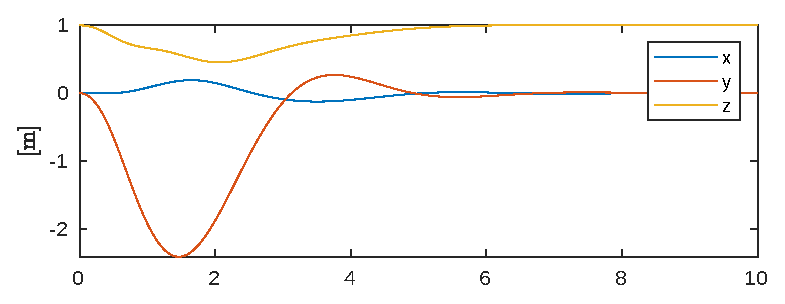
\includegraphics[width=0.8\linewidth]{fig/pos_edf}
    \caption{Posición del vehículo}
    \label{fig:pos_edf}
\end{figure}

\begin{figure}[!ht]
    \centering
    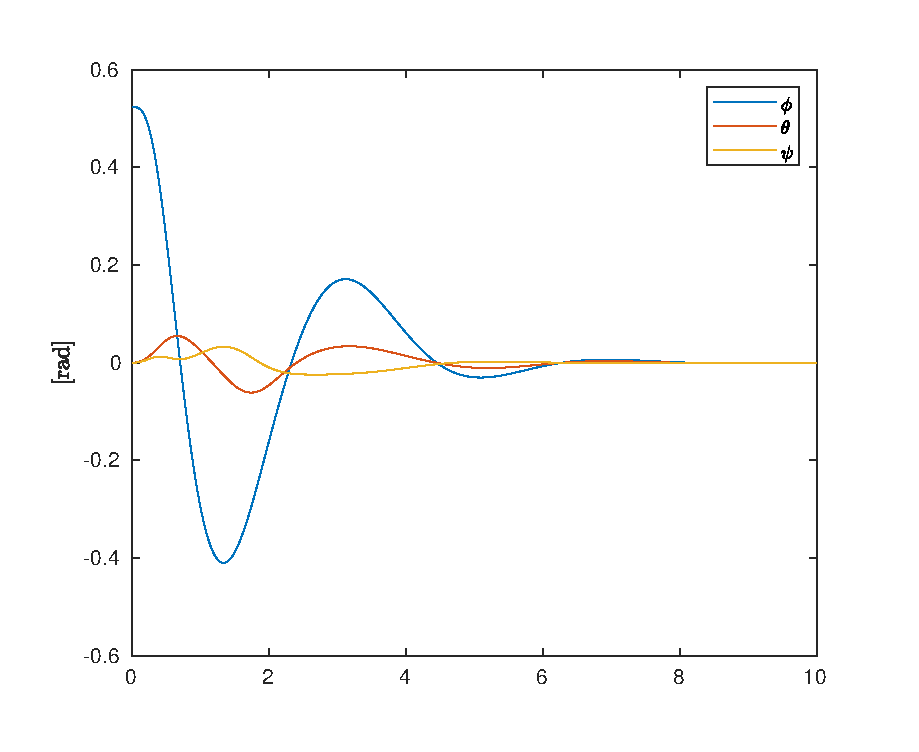
\includegraphics[width=0.6\linewidth]{fig/eulerang_edf}
    \caption{Ángulos de euler. Note que solo hubo perturbación inicial en $\phi$ sin embargo la actuación del gimbal ($\alpha$) generó una perturbación interna en $\theta$ por el efecto giroscópico.}
    \label{fig:eulerang_edf}
\end{figure}

\begin{figure}[!ht]
    \centering
    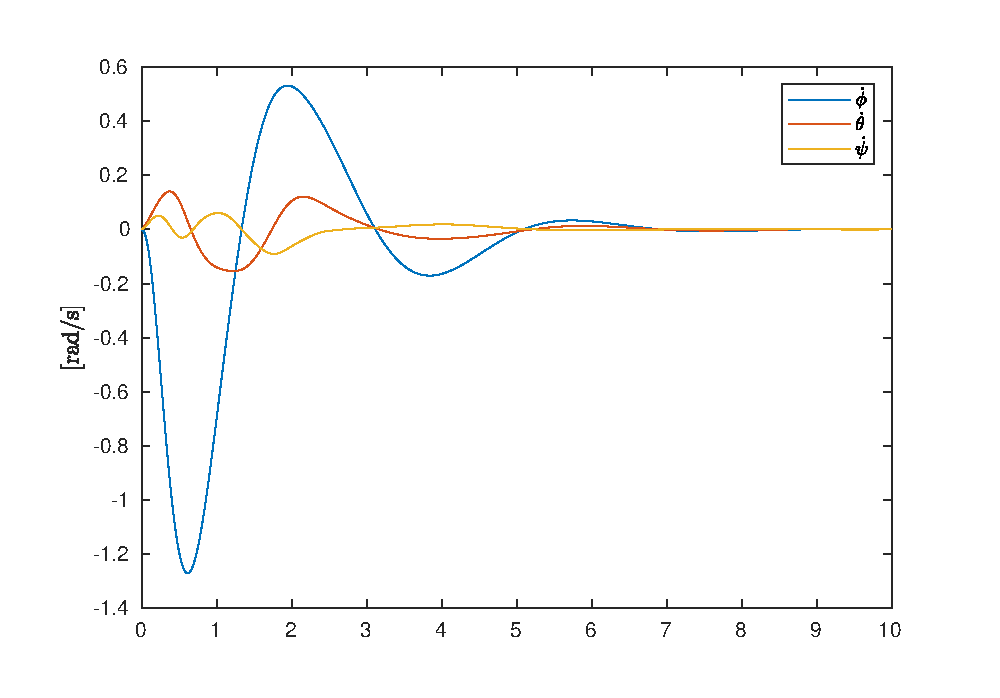
\includegraphics[width=0.6\linewidth]{fig/angvel_edf.eps}
    \caption{Velocidad angular del vehículo}
    \label{fig:angvel_edf.eps}
\end{figure}

\begin{figure}[!ht]
    \centering
    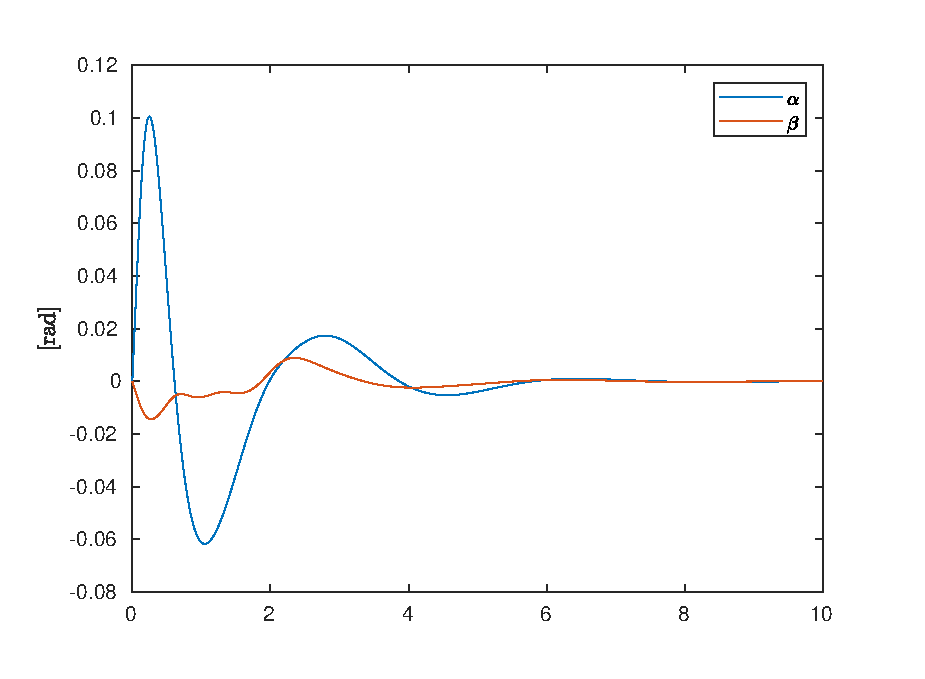
\includegraphics[width=0.6\linewidth]{fig/actuator_edf}
    \caption{Actuación angular del gimbal.}
    \label{fig:actuator_edf}
\end{figure}

\begin{figure}[!ht]
    \centering
    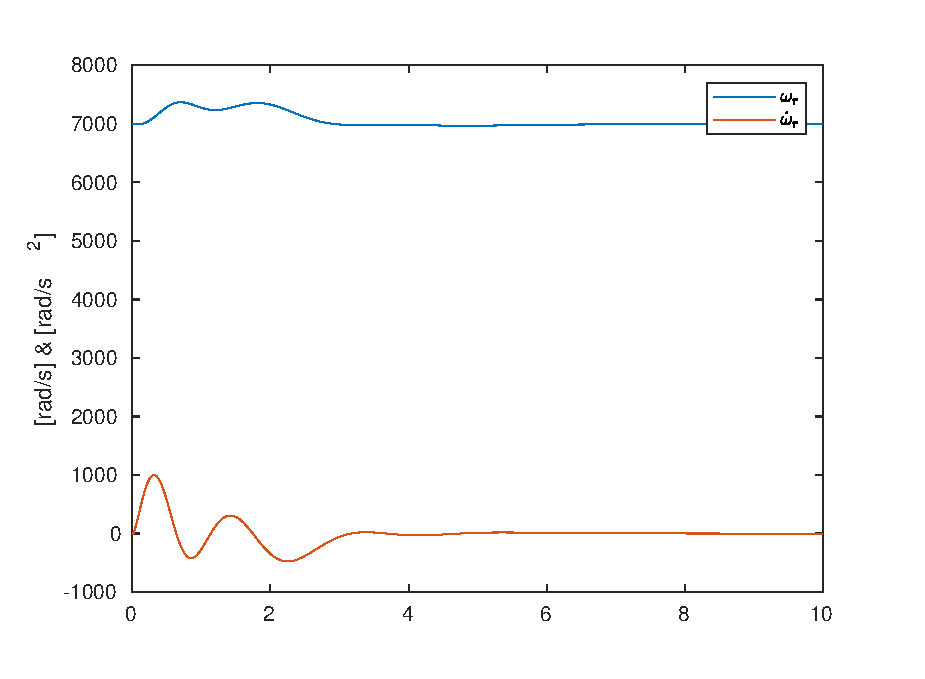
\includegraphics[width=0.6\linewidth]{fig/rotor_edf}
    \caption{Velocidad y aceleración angular del rotor.}
    \label{fig:rotor_edf}
\end{figure}



